\documentclass[10pt]{article}

\def\Type{LessonDJ}
\def\TypeNum{Workshop Week 7} %Lesson #
\def\TypeTitle{First and Second  Derivatives } %Lesson Title
\def\Semester{Fall 2021} %Not Used 
\def\Course{MATH 1190}%Course number and name
\def\Targets{ \target{A1}, \target{A2} }

\usepackage{preambleDJ} 

%%%%%%%%%%%% BEGIN DOCUMENT %%%%%%%%%%%%%%%
%%%%%%%%%%%% BEGIN DOCUMENT %%%%%%%%%%%%%%%
%%%%%%%%%%%% BEGIN DOCUMENT %%%%%%%%%%%%%%%
%%%%%%%%%%%% BEGIN DOCUMENT %%%%%%%%%%%%%%%
%%%%%%%%%%%% BEGIN DOCUMENT %%%%%%%%%%%%%%%

\begin{document}
\pagestyle{otherpages}
\thispagestyle{firstpage}

\vs{.6}
The following are test questions from the Fall 2023 \& Fall 2024 semesters.

%\begin{enumerate}
%
%\item ({\bf\color{ForestGreen}D2}) Find the first and second derivatives of $f(x) = x^3 - 3x^2$. Construct the sign chart for $f'$ and $f''$. For what values of $x$ does $f'(x) = 0$? For what values of $x$ does $f''(x) = 0$? What do these points represent?
%
%    \vfill
%
%% \item ({\bf\color{ForestGreen}D3}) Record the derivatives of the following functions. You may simply write your answers without showing any work. 
%
%% {\bf If you do need to show some work, then please do so on the bottom half of the page -- not on the answer spaces.}\\
%
%\end{enumerate}

% \begin{center}

%         \begin{tabular}{l c r l c r}
%             %
%             $\displaystyle\frac{d}{dx}\left[ \ln(2) \right]$ & $=$ & \rule[-8pt]{2in}{0.4pt} &
%             %
%             $\displaystyle\frac{d}{dx}\left[ \left(\frac{1}{2}\right)^x \right]$ & $=$ & \rule[-8pt]{2in}{0.4pt}\\[0.3in]
%             %%%%%
%             $\displaystyle\frac{d}{dx}\left[ \frac{1}{\sqrt{x^5}} \right]$ & $=$ & \rule[-8pt]{2in}{0.4pt} & 
%             %
%             $\displaystyle\frac{d}{dx}\left[ e^5 \right]$ & $=$ & \rule[-8pt]{2in}{0.4pt}\\[0.3in]
%             %%%%%
%             $\displaystyle\frac{d}{dx}\left[ \log_4(x) \right]$ & $=$ & \rule[-8pt]{2in}{0.4pt} &
%             % 
%             $\displaystyle\frac{d}{dx}\left[ \ln(x) \right]$ & $=$ & \rule[-8pt]{2in}{0.4pt}\\[0.3in]
%             %%%%%
%             $\displaystyle\frac{d}{dx}\left[ \sqrt[3]{x} \right]$ & $=$ & \rule[-8pt]{2in}{0.4pt} & 
%             %
%             $\displaystyle\frac{d}{dx}\left[ \frac1x \right]$ & $=$ & \rule[-8pt]{2in}{0.4pt}\\[0.3in]
%             %%%%%
%         \end{tabular}

% \vspace{1in}

% \end{center}




%%%%%%%%%%%%%%%%%%%%%%%%%%%%%%%%%%%%%%%%%%%%%%
%%% PUT BOARDWORK PROBLEMS AFTER THIS NOTE! %%
%%%%%%%%%%%%%%%%%%%%%%%%%%%%%%%%%%%%%%%%%%%%%%

\section{Conceptual Critical Number and Inflection Points}


Let $f(x)$ be the function represented by the following graph:\\
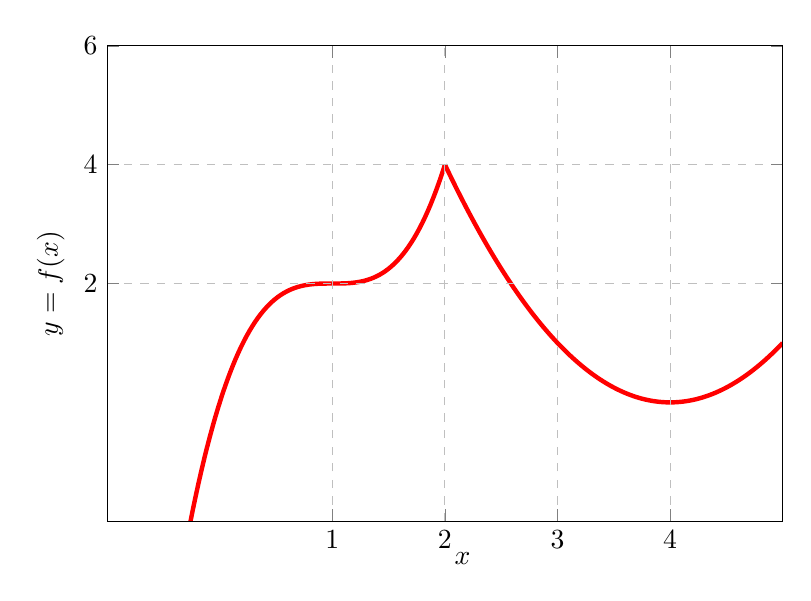
\begin{tikzpicture}[scale=1]
          \begin{axis}[
        %    axis y line = left,
        %    axis x line = bottom,
            xlabel={$x$},
            xtick       = {2,4,6,8},
            xticklabels = {1,2,3,4},
            ytick       = {2,4,6,8,10,12},
            %yticklabels = {,$1.75$,$4$},
            samples     = 160,
            xmin = -2, xmax = 10,
            ymin = -2, ymax = 6,
            restrict y to domain=-20:20,
            grid=both, grid style=dashed,
            width=4in, height=3in,
            y label style={anchor=south},
            ylabel={$y=f(x)$},
        		axis on top,
		x label style={anchor=west},
          ]
%\addplot[red, ultra thick, domain=-4:3.9] {-((x-2)^3)/(x-4) + 2};
\addplot[red, ultra thick, domain=-4:4] {1/4*(x-2)^3+ 2};
\addplot[red, ultra thick, domain=4:10] {1/4*(x-8)^2};
%\addplot[red, ultra thick,, domain=4.05:6] {.25*((x-9)*(x-6)^2)/(-(x-4))};
%\addplot[red, ultra thick,, domain=6:8] {((x-9)*(x-6)^2)/(-(x-4))};

%\addplot[red, ultra thick,, domain=8:10] {(x-8)^3 + 1};
        % Open circle for the limit from the left
%\filldraw[black, fill=white] (axis cs:8,1) circle (1.5pt);
%        % Solid dot for the defined value at x=8
%        \filldraw[black] (axis cs:8,0) circle (1.5pt);
        \end{axis}
        \end{tikzpicture}
        
        \begin{enumerate}
    \item Find all the critical numbers of $f$.

    \item At which critical number(s) does $f$ attain local extrema? Find the intervals where $f$ is increasing or decreasing.

    \item Find all the inflection points of $f$.
    \item Find the intervals where $f$ is concave up and concave down
\end{enumerate}

\newpage

\section{Critical Points, Increasing and Decreasing, First Derivative}

\begin{enumerate}
    \item Let $f(x) = x^3 - 6x^2 + 9x - 4$. Compute $f'$. 
    \item Find the critical points of $f(x)$. 
    \item Construct the sign chart for $f'$. On what intervals is $f$ increasing, and on what intervals is $f$ decreasing? 
    \item Find $f''$. 
    \item Construct the sign chart for $f''$ On what intervals is $f$ concave up and concave down?
    \item Try to use the information you have found so far to graph $f$. You may find it useful to know that $x^3 - 6x^2 + 9x - 4 = (x-1)^2(x-4)$.
\end{enumerate}

\newpage

\section{More Critical Points, Increasing and Decreasing, First Derivative}

\begin{enumerate}
    \item Let $g(x) = \frac{1}{x^2 + 4}$. Compute $g'$. 
    \item Find the critical points of $g(x)$. 
    \item Construct the sign chart for $g'$. On what intervals is $g$ increasing, and on what intervals is $g$ decreasing? 
    \item Does $g$ have any local maxima or minima? What are they?
    \item Find  $g''$
    \item Construct the sign chart for $g''$.  When is $g$ concave up and when is $g$ concave down?
    \item Try to use the information you have found so far to graph $g$. 
\end{enumerate}

\newpage




\section{Even More Critical Points, Increasing and Decreasing, First Derivative}
\begin{enumerate}
    \item Let $h(x) = \sqrt{4 - x^2}$. Compute $h'$.
    \item What is the $y$-intercept of $h$? What are the zeros of $h$?
    \item Compute $h'$ and find the critical points of $h$. 
    \item Construct the sign chart for $h'$. On what intervals is $h$ increasing, and on what intervals is $h$ decreasing? 
    \item Does $h$ have any maxima or minima? What are they?
    \item Try to use the information you have found so far to graph $h$. Can you recognize what shape the graph of $h$ is merely from the formula? 
\end{enumerate}
\newpage


\section{Lots More Critical Points, Increasing and Decreasing, First Derivative}
\begin{enumerate}
    \item Sketch a graph of $f(x)=x^{2}-\ln(x).$ You may use technology if you wish. Note that $\ln(x)$ is only defined for $x > 0$. 
    \item Compute the critical points of $f(x)=x^{2}-\ln(x).$ Do each step in detail. 
    \item Find the critical points and create a sign chart for $f'$
    \item On what intervals is this function increasing, on which is it decreasing? 
    \item On which interval does the function attain a local maximum/minimum?
    \item When is $f(x)$ concave up? When is $f(x)$ concave down? 
\end{enumerate}

\newpage

\section{Challenge problem: Conceptual Critical Number and Inflection Points}


Let $f(x)$ be the function represented by the following graph:\\
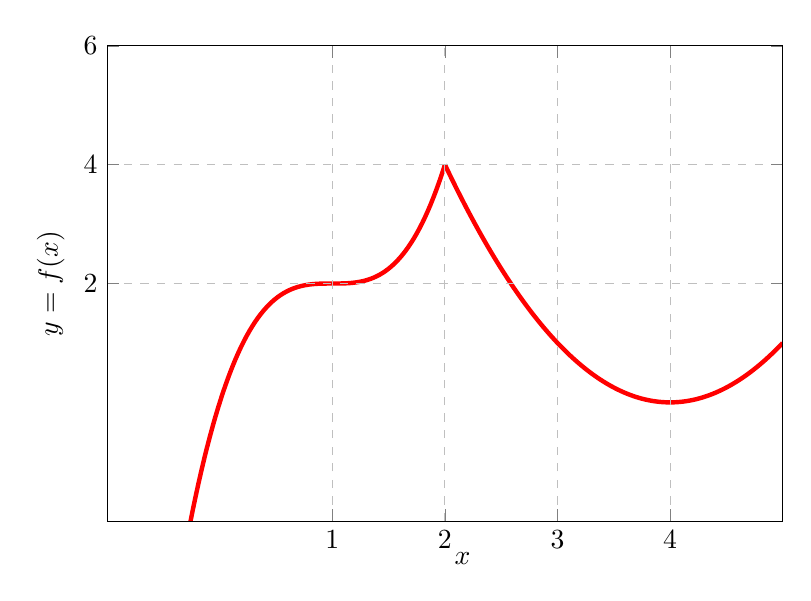
\begin{tikzpicture}[scale=1]
          \begin{axis}[
        %    axis y line = left,
        %    axis x line = bottom,
            xlabel={$x$},
            xtick       = {2,4,6,8},
            xticklabels = {1,2,3,4},
            ytick       = {2,4,6,8,10,12},
            %yticklabels = {,$1.75$,$4$},
            samples     = 160,
            xmin = -2, xmax = 10,
            ymin = -2, ymax = 6,
            restrict y to domain=-20:20,
            grid=both, grid style=dashed,
            width=4in, height=3in,
            y label style={anchor=south},
            ylabel={$y=f(x)$},
        		axis on top,
		x label style={anchor=west},
          ]
%\addplot[red, ultra thick, domain=-4:3.9] {-((x-2)^3)/(x-4) + 2};
\addplot[red, ultra thick, domain=-4:4] {1/4*(x-2)^3+ 2};
\addplot[red, ultra thick, domain=4:10] {1/4*(x-8)^2};
%\addplot[red, ultra thick,, domain=4.05:6] {.25*((x-9)*(x-6)^2)/(-(x-4))};
%\addplot[red, ultra thick,, domain=6:8] {((x-9)*(x-6)^2)/(-(x-4))};

%\addplot[red, ultra thick,, domain=8:10] {(x-8)^3 + 1};
        % Open circle for the limit from the left
%\filldraw[black, fill=white] (axis cs:8,1) circle (1.5pt);
%        % Solid dot for the defined value at x=8
%        \filldraw[black] (axis cs:8,0) circle (1.5pt);
        \end{axis}
        \end{tikzpicture}
        


Let us define a new function $g(x) = (f(x))^2 + 1$ that depends on the above function $f$.
\begin{enumerate}
    \item Compute $g'(x)$. Your answer will contain $f(x)$ and $f'(x)$.
    \item Find the critical numbers for $g(x)$. 
        \item Write down  all the inflection points of $f$ from Section 1.
    \item Compute $g''(x)$. your answer will contain $f(x)$, $f'(x)$ and $f''(x)$ 
    \item What is the concavity of $g$ at $x = 0$ (Hint: What is the sign of $g(x)$ when you plug $x = 0$ into $g''(x)$?)
    \item Is it possible that  the inflection points of $f$ might also be inflection points of $g$?  What happens if you plug the inflection points of $f$ into $g''(x)$? Why or why not?
\end{enumerate}




\end{document}